\section{Model and conventions}\label{sec:model}

\subsection{Beams}
The scalar paraxial donut is the LG$_{01}$ intensity in the parametrization of Balzarotti
Eq.~S17 \cite{Balzarotti2017}, normalized to a ring peak of one:
\begin{equation}
\begin{aligned}
I_{\mathrm{LG}}(\rho)&=4e\ln2\,\frac{\rho^2}{\fwhm^2}\exp\!\Big(-4\ln2\,\frac{\rho^2}{\fwhm^2}\Big)\\
&\equiv e\,a\rho^2e^{-a\rho^2},\qquad a=\frac{4\ln2}{\fwhm^2}.
\end{aligned}
\label{eq:lg}
\end{equation}
Here $\fwhm$ is a \emph{size parameter}, not the full width at half maximum of any curve of the
donut: the ring has a peak-to-peak diameter $\fwhm/\sqrt{\ln2}$, i.e.\
\pnum{lg_ring_diameter_nm}\src{lg_ring_diameter_nm}\,nm for our default
$\fwhm=\pnum{fwhm_nm}\src{fwhm_nm}$\,nm. Near the zero $I_{\mathrm{LG}}\simeq ea\rho^2$
(quadratic).

The vectorial donut is computed with the Richards--Wolf (Debye) integral for an aplanatic
objective \cite{Caprile2022}: a Gaussian beam with a $0$--$2\pi$ vortex phase $e^{i\phi}$ and
circular polarization, focused with wavelength $\lambda=640$\,nm, numerical aperture
$\mathrm{NA}=1.4$, refractive index $n=1.518$ and filling factor $5/3$; the intensity is
$|E_x|^2+|E_y|^2+|E_z|^2$. We call ``correct'' the handedness for which the circular polarization
rotates in the same sense as the phase ramp \cite{Lopez2023,Caprile2022}; in our formulation,
the product of the topological charge and the photon spin is $+1$. Figure~\ref{fig:schematic}(a,b)
compares the profiles.

\subsection{Triangular coordinate pattern}
Following Balzarotti Eq.~S24 \cite{Balzarotti2017}, up to a global rotation and a relabelling
of the exposures (centre last), the TCP has $K=4$ exposures with zeros at
\begin{equation}
\begin{gathered}
\bb_k=\frac{L}{2}\,(\cos\varphi_k,\sin\varphi_k),\qquad \varphi_k=\frac{\pi}{2}+\frac{2\pi k}{3},\\
k=0,1,2,\qquad \bb_3=\mathbf{0},
\end{gathered}
\label{eq:tcp}
\end{equation}
so that $L$ is the \emph{diameter} of the circle of peripheral zeros
[Fig.~\ref{fig:schematic}(c)]. Each exposure uses the same beam displaced to $\bb_i$,
$I_i(\rr)=I(|\rr-\bb_i|)$.

\subsection{Photon statistics, background and SBR}
For a fixed total number $N$ of detected photons the counts $(n_0,\dots,n_3)$ are multinomial
with probabilities \cite{Balzarotti2017}
\begin{equation}
\begin{gathered}
p_i^{(0)}(\rr)=\frac{I_i(\rr)}{\sum_jI_j(\rr)},\\
p_i(\rr)=\frac{\sbr}{\sbr+1}\,p_i^{(0)}(\rr)+\frac{1}{\sbr+1}\,\frac1K,
\end{gathered}
\label{eq:p}
\end{equation}
where the second form (Balzarotti Eq.~S30) adds a background equal in all exposures. The SBR is
the total signal over the total background summed over the $K$ exposures at the emitter position
(Eq.~S29), so for a fixed background it depends on the position and on the pattern. In all our
simulations, however, we hold the SBR fixed at the quoted value at every position (Eq.~S30 with
constant SBR), which implies a position-dependent background; with a fixed background the SBR
would instead vary with position (Eq.~S29) and, at the centre, fall as $L$ decreases (Eq.~S32). When the beam carries a pedestal
(finite zero depth, Sec.~\ref{sec:nonideal}) the SBR refers to the signal of the full beam,
pedestal included. For the camera (Sec.~\ref{sec:camera}) we use Balzarotti's $\sbr_c$, total
signal over the background \emph{per pixel}.

\subsection{Fisher information and CRB}
The Fisher information for the emitter position is
\begin{equation}
F(\rr)=N\sum_{i=0}^{K-1}\frac{\nabla p_i\,\nabla p_i^{T}}{p_i},
\label{eq:fisher}
\end{equation}
and we report the per-axis bound
\begin{equation}
\crb=\sqrt{\tfrac12\,\mathrm{tr}\,F^{-1}},
\label{eq:crb}
\end{equation}
Balzarotti's Eq.~S13. The MC precision uses the same convention,
$\sigma=[(\mathrm{var}\,\hat x+\mathrm{var}\,\hat y)/2]^{1/2}$, and the root-mean-square error
is $\mathrm{rmse}=[\langle|\hat\rr-\rr|^2\rangle/2]^{1/2}$. At the exact centre of the TCP
without background the central exposure has $p_3=0$ and Eq.~\eqref{eq:fisher} is ill defined;
Sec.~\ref{sec:crb} distinguishes the \emph{point value} at $r=0$ from the \emph{limit}
$r\to0$, and ``centre CRB'' means the limit unless stated otherwise.

\subsection{Estimators}
The MLE maximizes $\sum_in_i\ln p_i(\rr)$ over a disk (grid search followed by a local
refinement). The disk radius is part of the protocol and is stated with each result: $L$ for
centre points, $2L$ for positions swept across the pattern, and $0.75L$ for the iterative and
misalignment studies. The LMS and modified LMS (mLMS) estimators are the linearized estimators
of Balzarotti Eqs.~S49--S51 \cite{Balzarotti2017}, the latter with the polynomial coefficients
$(1.27,3.8)$ used there for live tracking.

\begin{figure*}[t]
\centering
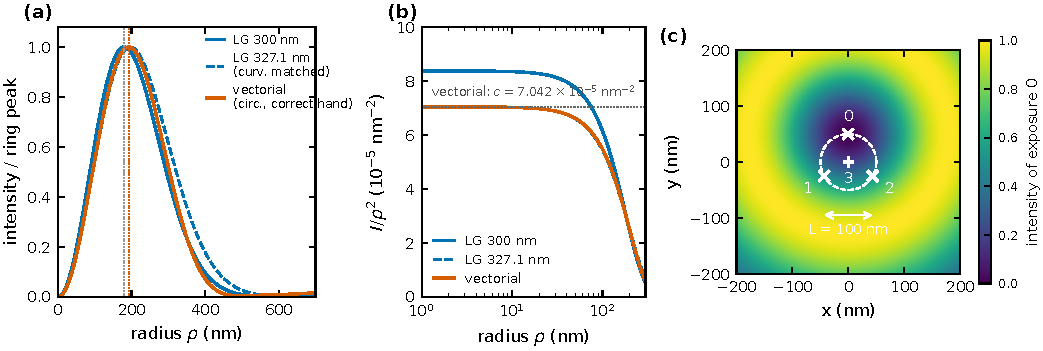
\includegraphics[width=\textwidth]{figures/fig1_schematic.pdf}
\caption{Beam model and TCP geometry. (a)~Normalized radial profiles of the scalar LG$_{01}$
donut ($\fwhm=\pnum{fwhm_nm}\src{fwhm_nm}$\,nm, Eq.~\ref{eq:lg}), of the LG donut with the zero
curvature of the vectorial donut ($\fwhm=\pnum{vectorial_lg_fwhm_curvature_nm}\src{vectorial_lg_fwhm_curvature_nm}$\,nm),
and of the vectorial Richards--Wolf vortex donut with circular polarization of the correct hand
($\lambda=640$\,nm, $\mathrm{NA}=1.4$, $n=1.518$, filling factor $5/3$); dotted lines mark the
ring radii, i.e.\ half the peak-to-peak diameters
\pnum{lg_ring_diameter_nm}\src{lg_ring_diameter_nm}\,nm (LG) and
\pnum{vectorial_peak_to_peak_diameter_nm}\src{vectorial_peak_to_peak_diameter_nm}\,nm
(vectorial). (b)~$I/\rho^2$ near the zero on a logarithmic radius axis: all zeros are quadratic,
the vectorial curvature is
$c=\pnum{vectorial_zero_curvature_nm2}\src{vectorial_zero_curvature_nm2}$\,nm$^{-2}$, and the
curvature-matched LG follows the vectorial profile for $\rho\lesssim100$\,nm. (c)~TCP: three
donut zeros ($\times$) on a circle of diameter $L$ (dashed; $L=100$\,nm shown for visibility)
plus a central exposure ($+$); the map is the intensity of exposure~0.}
\label{fig:schematic}
\end{figure*}
